\documentclass{article}

\usepackage{graphicx}
\usepackage{tikz}
\usepackage{tikzsymbols}
\usetikzlibrary{calc,patterns,shapes.geometric}
\pagestyle{empty}
\usepackage[margin=0pt]{geometry}
\geometry{papersize={14in,12in}}

\def\centerarc[#1](#2)(#3:#4:#5){\draw[#1] ($(#2)+({#5*cos(#3)},{#5*sin(#3)})$) arc (#3:#4:#5);}

\begin{document}
	\begin{figure}
		\centering
		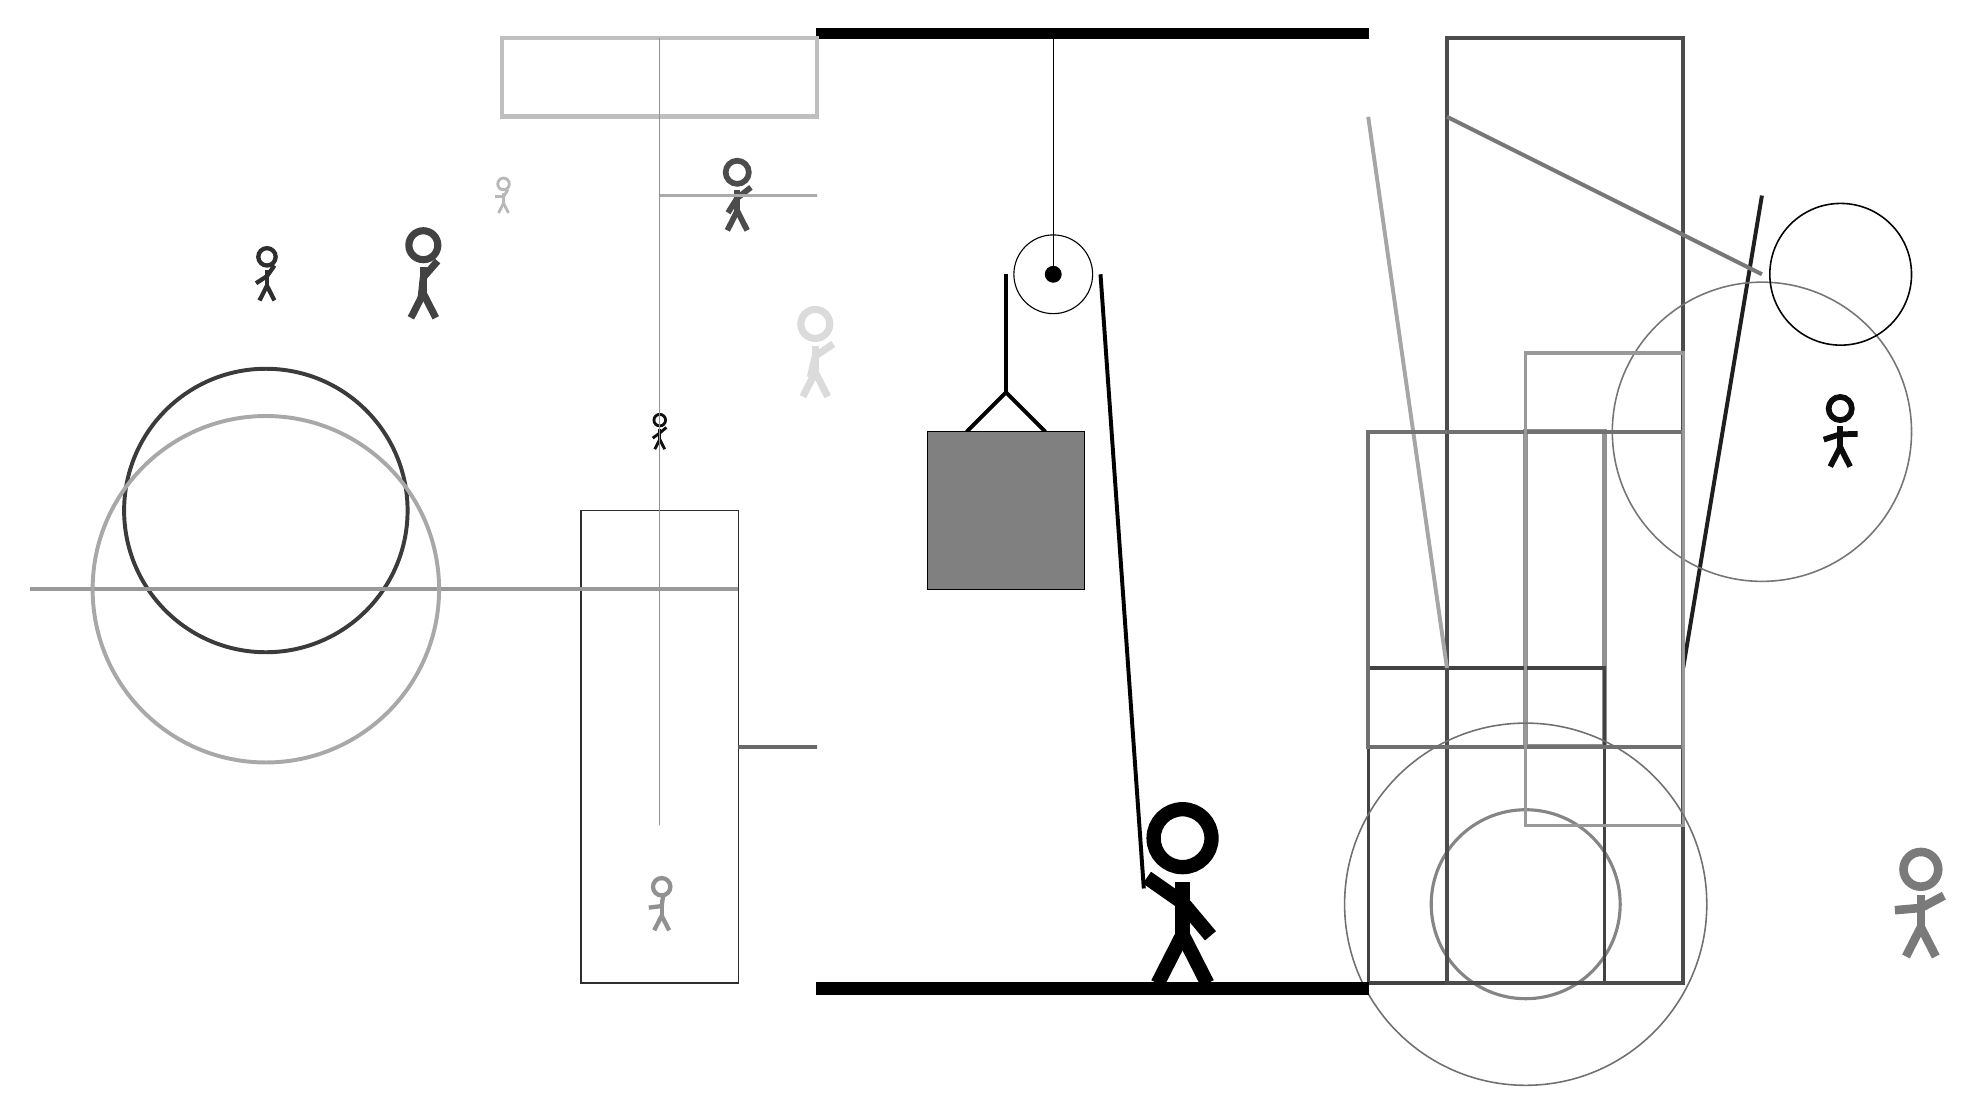
\begin{tikzpicture}
			%%%%% START %%%%%
			
			\draw[fill=black] (-2, 9) rectangle (5, 9.125);
			
			\draw (1, 6) circle (0.5);
			\draw[fill=black] (1, 6) circle (0.1);
			\draw (1, 9) -- (1, 6);
			
			\draw[line width=0.5mm] (-0.1, 4.0) -- (0.4, 4.5) -- (0.9, 4.0);
			\draw[fill=black!50] (-0.6, 4.0) rectangle (1.4, 2.0);
			
			\node[line width=0.5mm, color=black!95] at (11, 4) {\Strichmaxerl[4][18][1]};
			
			\draw [line width=0.5mm, color=black!77](-9, 3) circle (1.8);
			\draw [line width=0.4mm, color=black!48](7, -2) circle (1.2);
			\draw[line width=0.6mm, color=black!43] (7, 4) rectangle (8, 0);
			\draw[line width=0.5mm, color=black!88](9, 1) -- (10, 7);
			
			\node[line width=0.4mm, color=black!14] at (-2, 5) {\Strichmaxerl[5][77][34]};
			
			\draw[line width=0.4mm, color=black!74] (5, 1) rectangle (8, -3);
			\draw[line width=0.5mm, color=black!70] (6, -3) rectangle (9, 9);
			\node[line width=0.3mm, color=black!82] at (-9, 6) {\Strichmaxerl[3][33][55]};
			\draw[line width=0.2mm, color=black!82] (-3, 3) rectangle (-5, -3);
			\node[line width=0.6mm, color=black!28] at (-6, 7) {\Strichmaxerl[2][0][59]};
			\node[line width=0.2mm, color=black!52] at (12, -2) {\Strichmaxerl[6][5][28]};
			\draw [line width=0.2mm, color=black!54](10, 4) circle (1.9);
			\node[line width=0.4mm, color=black!94] at (-4, 4) {\Strichmaxerl[2][36][40]};
			\draw[line width=0.5mm, color=black!59] (-3, 0) rectangle (-2, 0);
			\node[line width=0.7mm, color=black!70] at (-3, 7) {\Strichmaxerl[4][58][38]};
			
			\draw[line width=0.5mm, color=black!35](5, 8) -- (6, 1);
			\node[line width=0.2mm, color=black!74] at (-7, 6) {\Strichmaxerl[5][84][49]};
			\node[line width=0.6mm, color=black!43] at (-4, -2) {\Strichmaxerl[3][7][82]};
			\draw[line width=0.6mm, color=black!25] (-2, 8) rectangle (-6, 9);
			\draw [line width=0.6mm, color=black!36](8, 1) circle (0.0);
			
			\draw[line width=0.3mm, color=black!33] (-2, 7) rectangle (-4, 7);
			\draw [line width=0.5mm, color=black!58](12, 0) circle (0.0);
			\draw [line width=0.2mm, color=black!99](11, 6) circle (0.9);
			\draw[line width=0.5mm, color=black!56] (5, 0) rectangle (9, 4);
			
			\draw[line width=0.4mm, color=black!40] (7, -1) rectangle (9, 5);
			
			\draw[line width=0.2mm, color=black!43] (-4, -1) rectangle (-4, 9);
			\draw[line width=0.5mm, color=black!40](-3, 2) -- (-12, 2);
			
			\draw [line width=0.5mm, color=black!34](-9, 2) circle (2.2);
			\draw [line width=0.2mm, color=black!56](7, -2) circle (2.3);
			\draw[line width=0.5mm, color=black!53](6, 8) -- (10, 6);
			
			\draw[line width=0.5mm] (0.4, 6) -- (0.4, 4.5);
			\centerarc[line width=0.5mm](1, 6)(0:180:0.6);
			\draw[line width=0.5mm](1.6, 6) -- (2.15, -1.8);
			
			\node at (2.6, -1.9) {\Strichmaxerl[10][-35][-50]};
			
			\draw[fill=black] (-2, -3) rectangle (5, -3.15);
			
			%%%%% END %%%%%
		\end{tikzpicture}
	\end{figure}	
\end{document}